\documentclass[a4paper,draft]{scrbook}
\usepackage{a4wide,amsmath}
\usepackage[final]{graphicx}
\usepackage[square,numbers]{natbib}
\usepackage[draft=false]{hyperref}  %% need this for links and references in the document
\usepackage{array}     %% need this for more table formating (m{} and p{})
\usepackage{url}       %% support for URLs
\usepackage{float}     %% required for extra float placement
\usepackage{xcolor}
\usepackage{placeins}
\usepackage{subfig}
\usepackage{lscape}    %% landscape figures
\usepackage{todonotes}
\usepackage{color}
\usepackage[figuresright]{rotating}
\usepackage{minted}    %% excellent source code formating
\usepackage{tikz}

\usetikzlibrary{trees,shapes.geometric,positioning,calc}

\definecolor[named]{desycyan}{rgb}{0,0.648,0.918}
\definecolor[named]{desyorange}{rgb}{0.945,0.555,0}
\definecolor[named]{desygray}{rgb}{0.465,0.465,0.465}
\definecolor[named]{desywhite}{rgb}{1,1,1}

\hypersetup{pdftitle={libpniio API review 2013 },
        	pdfborder=0 0 0,
	    	colorlinks=false}

\setcapindent{0em}

\title{{\Huge{\tt libpniio} Users Guide}}
\author{Eugen Wintersberger}

\newcommand{\libpnicore}{\texttt{libpnicore}}
\newcommand{\libpniio}{\texttt{libpniio}}
\newcommand{\sdarray}{\texttt{static\_array}}
\newcommand{\darray}{\texttt{dynamic\_array}}
\newcommand{\farray}{\texttt{fixed\_dim\_array}}
\newcommand{\mdarray}{\texttt{mdarray}}
\newcommand{\arrayview}{\texttt{array\_view}}
\newcommand{\arrayerasure}{\texttt{array}}
\newcommand{\numarray}{\texttt{numeric\_array}}
\newcommand{\cmake}{\texttt{cmake}}
\newcommand{\pkgconfig}{\texttt{pkg-config}}
\newcommand{\gcc}{\texttt{gcc}}
\newcommand{\nxfield}{\texttt{nxfield}}
\newcommand{\nxobject}{\texttt{nxobject}}
\newcommand{\nxgroup}{\texttt{nxgroup}}
\newcommand{\nxattribute}{\texttt{nxattribute}}
\newcommand{\nxfile}{\texttt{nxfile}}
\newcommand{\nxpath}{\texttt{nxpath}}
\newcommand{\cpp}[1]{\texttt{#1}}
\newcommand{\nexus}{NeXus}

%\bibliographystyle{plainnat}

\newminted{cpp}{fontsize=\small}
\newminted{xml}{fontsize=\small}

\begin{document}
\maketitle
\tableofcontents
\listoftodos

%%%---------------------------------------------------------------------------
\chapter{Introduction}\label{chapter:introduction}
%%% a general introduction to libpniio

\libpniio\ is the IO library within the PNI library stack. More precisely it is
responsible for file IO. Although several legacy formats are supported the
library mainly deals with Nexus files providing functions and objects to deal
with these kind of files. 

Chapter~\ref{chapter:legacy_formats} gives an overview over the supported legacy
formats and how to access data. It is important to note that the legacy support
is mainly for reading data. The reason for this is that newly created data
should be written as Nexus files. 

Chapter~\ref{chapter:nexus_quickstart} gives a quick overview over Nexus and
provides a kind of quick start tutorial how to use the library. 
In the ongoing chapters present more detailed information about how to work with
Nexus files with \libpniio.




\FloatBarrier

%%%---------------------------------------------------------------------------
\chapter{Installation}\label{chapter:installation}
%%% describe the installation procedure


\section{Install precompiled packages}

\section{Install from sources}

\subsection{Running tests}

In order to run the tests use 
\begin{minted}{bash}
> make cleanup test
\end{minted}
The \cpp{cleanup} target removes the test artifacts from previous test runs.
This is important as some of the tests may fail if the old artifacts are still
present.

\FloatBarrier

%%%---------------------------------------------------------------------------
\chapter{Using the library}\label{chapter:usage}
%%%describing the usage of the library

In this section we will have a short look on how to make your code working the
\libpniio. The key to make using \libpniio\ simple is the usage of {\tt
pkg-config}. The rational behind the design descission to focus on {\tt
pkg-config} as the central element for build systems is simple: it works for
virtually all build systems. It is even available for Windows (though not very
often used). 

\section{From the command line}

\begin{minted}{bash}
    $> g++ -std=c++11 -otest test.cpp $(pkg-config --cflags --libs pniio)
\end{minted}
There are two important remarks we have to make here. The first is the {\tt
-std=c++11} after {\tt g++}. This tells the compiler to use the new C++11
standard. This option is absolutely required for the code to build. 
the {\tt pkg-config} command at the end of the command line includes all the
necessary compiler and linker flags to build and link the code.

\section{From within a Makefile}

{\tt pkg-config} can be used in a Makefile by putting the following at the top
of your Makefile
\begin{minted}{make}
CPPFLAGS=-O2 -g -std=c++11 $(shell pkg-config --cflags pniio)
LDFLAGS=$(shell pkg-config --libs pniio)
\end{minted}

\section{With CMake}

For {\tt cmake} the {\tt FindPkgConfig} module provides access to the
functionality of {\tt pkg-config}. The following snippet from a {\tt
CMakeLists.txt} file shows how to use it for \libpniio
\begin{minted}{cmake}
#load pkg-config package
include(FindPkgConfig)

#search for the pniio library 
pkg_search_module(PNIIO REQUIRED pniio)
link_directories(${PNIIO_LIBRARY_DIRS})
include_directories(${PNIIO_INCLUDE_DIRS})
add_definitions(${PNIIO_CFLAGS})

set(SOURCE ...)

add_executable(myprog ${SOURCE})
target_link_libraries(myprog ${PNIIO_LIBRARIES})
\end{minted}

\section{Dealing with updates and bug fixes}

Like \libpnicore, \libpniio\ is for most of its parts a template library. This
ensures good performance but comes at a price. Unlike binary only libraries
programs have to be rebuilt when a new version of \libpniio\ shall be used. 


\FloatBarrier

%%%---------------------------------------------------------------------------
\chapter{Legacy format support}\label{chapter:legacy_formats}
%%%-------------------------------------

The term legacy data refers to all non-Nexus file formats.
\libpnicore\ distinguishes between tow families of legacy formats 
\begin{itemize}
\item ASCII file where the content is entirely stored in human readable ASCII
characters
\item and binary data where the raw binary information is stored in a file.
\end{itemize}

%%%===========================================================================
\section{ASCII data}

\subsection{Lowlevel parser interface}

\libpniio\ provides a low level parser interface based on the \texttt{boost::spirit}
spirit framework. The major job of this interface is to provided save number
parsing. It supports all primitive data types provided by \libpnicore\ along
with \texttt{std::vector} begin a container of a primitive type.
For a detailed explanation about the low level parsers see
Appendix~\ref{appendix:parsers}. 

At the heart of the parser API is the \cpp{parser} class template. 
It takes one template parameter which is the primitive or container type 
to parse. To use the parser API just include \cpp{pni/io/parsers.hpp} in 
your source file. 

\subsubsection{Parsing primitive scalars}

A very simple example would be something like this
\begin{cppcode}
#include <iostream>
#include <pni/core/types.hpp>
#include <pni/io/parsers.hpp>

using namespace pni::core;
using namespace pni::io;

typedef parser<float64> float64_parser_type;

int main(int argc,char **argv)
{
    float64_parser_type p;

    float64 data = p("1.234");
    std::cout<<data<<std::endl;

    return 0;
}
\end{cppcode}
This example should be rather self explaining. 
When used with scalar values the parser template provides only a default 
constructor. No additional information is required to configure the 
parser code. 

Besides primitive types the \cpp{parser} template can also be used with 
the \cpp{value} type erasure. In this case the resulting parser matches 
either a \cpp{int64}, a \cpp{float64}, or a \cpp{complex64} type. Again 
no additional configuration at parser instantiation is required. 
For the ASCII representation of complex numbers see
Appendix~\ref{appendix:parsers}.

\subsubsection{Parsing a vector of primitives}

Besides single scalars the \cpp{parser} template can also be used with 
\cpp{std::vector} based containers where the element type should be one 
of the primitive types or a value. 
For this purpose a specialization of the \cpp{parser} template of the 
form
\begin{cppcode}
template<typename T> class parser<std::vector<T>> {...};
\end{cppcode}
is provided.
A particularly interesting choice as an element is the \cpp{value} type
erasure as it allows to parse a series of inhomogeneous types.
The following program
\begin{cppcode}
#include <iostream>
#include <vector>
#include <pni/core/types.hpp>
#include <pni/io/parsers.hpp>

using namespace pni::core;
using namespace pni::io;

typedef std::vector<value> record_type;
typedef parser<record_type> record_parser;

int main(int argc,char **argv)
{
    record_parser p;
    record_type data = p("1.234  12 1+I3.4");
    for(auto v: data)
        std::cout<<v.type_id()<<std::endl;

    return 0;
}
\end{cppcode}
would produce this output
\begin{verbatim}
FLOAT64
INT64
COMPLEX64
\end{verbatim}
When using the default constructor of the \cpp{parser} template with a 
container type the individual elements are considered to be separated by 
at least one blank. 
However the vector parser specialization
of the \cpp{parser} template provides three more additional constructors. 
The first, \cpp{parser(char del)} allows to use a custom delimiter symbol.
In the next example the \cpp{','} is used as a delimiter for the individual 
elements
\begin{cppcode}
record_parser p(',');
record_type data = p("1.234,12 , 1+I3.4");
\end{cppcode}
It is important to not that the delimiter symbol can be surrounded by an
arbitrary number of blanks. 
The second constructor provides the constructor with additional 
start and stop symbols. 
\begin{cppcode}
record_parser p('[',']');
record_type data = p("[1.234 12  1+I3.4]");
\end{cppcode}
However, the elements in the string are now again separated only by blanks. 
Full customization of the parser is provided by the third constructor which
allows the user to provide not only start and stop symbols but also a custom 
delimiter symbol
\begin{cppcode}
record_parser p('[',']',';');
record_type data = p("[1.234;12 ; 1+I3.4]");
\end{cppcode}

%%%===========================================================================
\section{Binary data}



\FloatBarrier

%%%---------------------------------------------------------------------------
\chapter{Getting started with \nexus}\label{chapter:nexus_quickstart}
%%% a basic introduction to Nexus

Today, data recorded during synchrotron experiments is typically stored in
individual binary image files and/or as flat ASCII files. 
Figure~\ref{fig:nxintro:old_fstree} shows the typicall directory structure of
such a setup. The ASCII file stores scalar data while the detector data is
stored in a separate directory as image files (here TIFF).
Such an approach leads to technical and organizational problems
\begin{enumerate}
\item when the number of image files grows large the performance of most file
systems degenerate 
\item to access data in an individual image file a new file handler has to be
created 
\item image and scalar data is stored in different files which increases the
managements efforts to keep related information aligned.
\end{enumerate}
\begin{figure}[tb]
    \centering
    \begin{minipage}[c]{0.4\linewidth}
    \centering
    \resizebox{\linewidth}{!}{\includegraphics{pics/old_fstree.pdf}}
    \end{minipage}
    \hspace{0.05\linewidth}
    \begin{minipage}[c]{0.5\linewidth}
    \caption{{\small A typical directory structure used at todays synchrotron
    experiments. Scalar data is stored in a single ASCII file while detector
    data is stored as individual image files in a separate directory.}}
    \label{fig:nxintro:old_fstree}
    \end{minipage}
\end{figure}

Nexus is a binary file format which attempts to solve all of these problems.
Nexus can keep scalar and multidimensional data within a single file and allows
to organize data in trees. Additional attributes can be attached to each object
in a file storing metadata which might be required for later analysis of the
data. It must be noted that Nexus is not a physical file format itself. It is
rather a set of rules how data must be organized within a particular format in
order to become a valid Nexus file. Currently the following physical file
formats are supported by the original Nexus API
\begin{itemize}
\item XML -- currently only used for file structure validation
\item HDF4 -- for historical reasons, should not be used for new data
\item HDF5 -- the current standard storage backend for Nexus files. 
\end{itemize}
One of the aims of \libpniio\ is to provide an abstraction layer between the
user and the storage backend. As \libpniio\ currently supports only HDF5 this is
rather artificial. However, \libpniio\ provides the architecture to include
other file formats to be used with Nexus too. 
There has been a lot of confusion what physical file format Nexus files are.
Many users think that Nexus has its own phyisical file format. This is in fact
not true. Just to avoid any further confusion fo the reader let me make this
clear once and for all
\begin{quote}
{\huge
{\color{red}Every Nexus file written by \libpniio\ is also a valid HDF5 file!}
\todo[caption={fix quote},inline]{This quote needs better formating. Maybe the
text should go into a box and the margins to the surrounding text must be
bigger}
}
\end{quote}

%%%===========================================================================
\section{The Nexus layer model}

\begin{figure}[tb]
    \centering
    \begin{minipage}[c]{0.4\linewidth}
    \centering
    \resizebox{\linewidth}{!}{\includegraphics{pics/nxlayers.pdf}}
    \end{minipage}
    \hspace{0.05\linewidth}
    \begin{minipage}[c]{0.5\linewidth}
    \caption{{\small Nexus can be considered to consist of three layers}}
    \label{fig:nxintro:layers}
    \end{minipage}
\end{figure}

\subsection{Layer 1 objects}

\begin{figure}[tb]
    \centering
    \begin{minipage}[c]{0.4\linewidth}
    \centering
    \resizebox{\linewidth}{!}{\includegraphics{pics/layer1.pdf}}
    \end{minipage}
    \hspace{0.05\linewidth}
    \begin{minipage}[c]{0.5\linewidth}
    \caption{{\small The basic objects of the first layer in the Nexus object
    model.}}
    \label{fig:nxintro:layer1}
    \end{minipage}
\end{figure}

\subsection{Layer 2 objects}

\subsection{Layer 3 objects}

\FloatBarrier

%%%---------------------------------------------------------------------------
\chapter{Addressing \nexus\ object - the \nexus-path}\label{chapter:nxpath}
%%% describing how to address Nexus objects

\newcommand{\fsection}{\textit{file section}}
\newcommand{\fsep}{\texttt{://}}
\newcommand{\osection}{\textit{object section}}
\newcommand{\asep}{\texttt{@}}
\newcommand{\asection}{\textit{attribute section}}
\newcommand{\nsection}{\textit{name section}}
\newcommand{\csection}{\textit{class section}}
\newcommand{\csep}{\texttt{:}}
\newcommand{\osep}{\texttt{/}}
\newcommand{\cgroup}{\texttt{.}}
\newcommand{\pgroup}{\texttt{..}}

%%%---------------------------------------------------------------------------
Objects within a \nexus-file can be referenced by a path. Though being very
similar to a Unix file system path, a \nexus-path provides much more
flexibility. It reflects one of the key features of \nexus: types. 
A \nexus-path can reference an object not only via its name (as HDF5 does) but
also by its type. Hence, under certain conditions, it is possible to construct
a path which is independent of the names choosen within a file.

%%%===========================================================================
\section{Introduction}
%%----------------------------------------------------------------------------
\begin{figure}[tb]
\centering
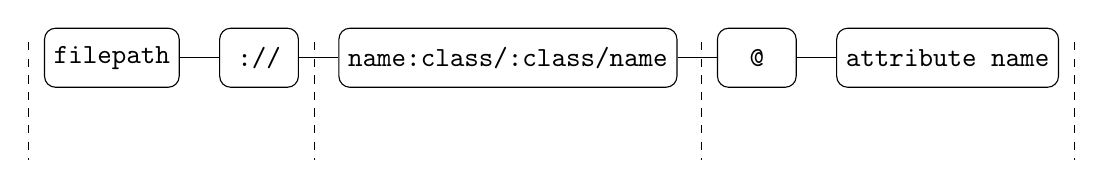
\begin{tikzpicture}
[cnode/.style = {rounded corners,draw=black,
                 minimum height = 0.75cm,
                 minimum width  = 1cm,
                 node distance = 0.5cm}]
\node (filenode) [cnode] {\texttt{filepath}};
\node (filesep)  [cnode,right = of filenode] {\texttt{://}};
\node (objnode)  [cnode,right = of filesep] {\texttt{name:class/:class/name}};
\node (attrsep)  [cnode,right = of objnode]  {\texttt{@}};
\node (attrnode) [cnode,right = of attrsep]  {\texttt{attribute name}};

\draw (filenode)--(filesep)--(objnode)--(attrsep)--(attrnode);

\draw[dashed] ($(filenode.west)+(-2mm,2mm)$) --
              node[below right=0.25cm and 0.75cm]{\fsection} 
              +(0,-1.5cm);
\draw[dashed] ($(filesep.east)+(2mm,2mm)$)  --
              node[below right=0.25cm and 1.5cm]{\osection}
              +(0,-1.5cm);
\draw[dashed] ($(attrsep.west)+(-2mm,2mm)$) --
              node[below right=0.25cm and 0.8cm]{\asection}
              +(0,-1.5cm);
\draw[dashed] ($(attrnode.east)+(2mm,2mm)$)  -- +(0,-1.5cm);

\end{tikzpicture}
\caption{\small\label{fig:path:structure}
The basic structure of a \nexus\ path as used by \libpniio. The \fsection\
stores the Unix path to the data file. The \osection\ the
path to the field or group within the file and the \asection\
holds the name of an attribute attached to the object referenced by the
previous path.
}
\end{figure}
%%----------------------------------------------------------------------------
\begin{figure}[tb]
\centering
\begin{minipage}[c]{0.6\linewidth}
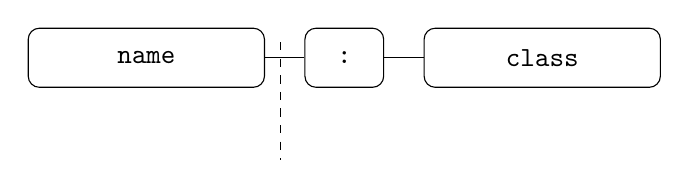
\begin{tikzpicture}
[cnode/.style = {rounded corners,draw=black,
                 minimum height = 0.75cm,
                 minimum width  = 1cm,
                 node distance = 0.5cm}]
\node (name) [cnode,minimum width=3cm] {\texttt{name}};
\node (sep)  [cnode,right = of name] {\texttt{:}};
\node (class) [cnode,right = of sep,minimum width=3cm] {\texttt{class}};
\draw (name) -- (sep) -- (class);

\draw[dashed] ($(name.east)+(2mm,2mm)$) -- 
              node[below right= 0.25cm and 1.4cm]{\csection}
              node[below left =0.25cm and 0.5cm]{\nsection}
              +(0,-1.5cm);

\end{tikzpicture}
\end{minipage}
\hfill
\begin{minipage}[c]{0.39\linewidth}
\caption{\small\label{fig:path:object} 
Structure of the elements in the \emph{object section} of a \nexus-path.
}
\end{minipage}
\end{figure}
%%%===========================================================================
\subsection{The structure of a \nexus-path}

Figure~\ref{fig:path:structure} shows the principal structure of a \nexus-path
as used by \libpniio. Such a path comprises three major sections
\begin{inlinetab}{m{0.2\linewidth}m{0.65\linewidth}}
 \emph{file section}      & which references the \nexus-file on the file system.
 It must thus be a valid file system path on the operating system platform in
 use.  \\
 \emph{object section}    & describing the location of an object within the file \\
 \emph{attribute section} & referencing an attribute attached to the object 
 pointed to by the residual path. The attribute is identified by its name.
\end{inlinetab}
As shown in Fig.~\ref{fig:path:structure} the file and the object sections are 
separated by \fsep\ while the object and attribute sections use \asep\ as a
delimiter. Both, the file and the attribute section, are optional.
 The individual elements in the object section are separated by a
single \osep. Every element in the \osection\ is composed of two parts
(see Fig.~\ref{fig:path:object}): the \nsection\ and the \csection 
separated by a \csep. Whether or not the \nsection\ and/or the \csection\ must
be present in order to reference an element depends on the circumstances. 
There are three possible situations
\begin{inlinetab}{m{0.15\linewidth}m{0.75\linewidth}}
\emph{name:class} & this is a full identifier for a group. It determines its
name as well as its type. As fields have no type they cannot be referenced by
such an expression. \\
\emph{name} & if only the name is given the referenced object can be either a
group or a field. However, in the case of a field, this must be the last element
in the object path (as fields cannot have additional children). \\
\emph{:class} & if only the class is given the referenced object must be a
group. Denote the leading colon in this expression. It is necessary to
distinguish such an expression from a mere name.
\end{inlinetab}

%%%===========================================================================
\subsection{Some general path properties}

A path is considered as \emph{absolute} if its \osection\ starts at the root
group of the file. This is always  the case if 
\begin{itemize}
\item the \fsection\ of the path is not empty
\item or, if no \fsection\ is given, the \osection\ starts with a leading \osep.
\end{itemize}
The latter condition is equivalent to the convention used for Unix file system
paths while the former requires some explanation. 
If the \fsection\ is not empty the \osection\ has to be considered absolute
otherwise we would not know where to start searching for objects. 
If no \fsection\ is provided the path can also be a relative path which
references an object relative to an already given parent object.
\todo{maybe we should present some example here}

The \nexus-path implementation provided by \libpniio\ also understands 
\cgroup\ and \pgroup\ where the former one refers to the current group while 
the latter one to the parent group of the current group.

%%%===========================================================================
\subsection{Examples}
Let's have a look on some examples. The following path addresses the data field 
in the detector group of a file
\begin{verbatim}
/data/run/detector.nxs://entry/instrument/detector/data
\end{verbatim}
Here, the individual groups are referenced by their name in the object section 
of the path. Indeed, this path can be written in a more general way with 
\begin{verbatim}
/data/run/detector.nxs://:NXentry/:NXinstrument/:NXdetector/data
\end{verbatim}
where the parent groups of the \cpp{data} field are referenced implicitly via
their type.  This requires that only one instance of a particular type
(\cpp{:NXentry}, \cpp{:NXinstrument}, etc.)  exists in its parent group. In the
case that we have two detectors and each of them is stored as an instance of
\cpp{NXdetector} below the \cpp{NXinstrument} group, the name of the detector
must be provided explicitly 
\begin{verbatim}
/data/run/detector.nxs://:NXentry/:NXinstrument/det1:NXdetector/data
\end{verbatim}
The last group reference \cpp{det1:NXdetector} is the most precise 
description of a group instance. Not only does it determined the name 
of the group but also its type.  This example already shows one of the 
powers of \nexus. As long as only one instance of a particular type exists
within a group it can be identified by its type rather than by its name. 
In many situations it is thus possible to generate paths which are virtually
independent of all object names (in fact only the fields must be named as they
have no type).

All path examples until now represented an absolute path (a path with a leading
\fsection). In many situations no file must be specified. A typical application
for paths without \fsection\ would be program where an object should be
referenced by a path relative to a given parent object. 
The path in the next example references the data field of the detector 
relative to the top level instance of \cpp{NXentry}
\begin{verbatim}
:NXinstrument/detector/data 
\end{verbatim}
In order to make a path without a \fsection\ \emph{absolute}, it must 
start with a leading \cpp{/} as in the next example
\begin{verbatim}
/:NXentry/:NXinstrument/pilatus/data
\end{verbatim}

In order to reference the root group of a file one can either use 
\begin{verbatim}
/
\end{verbatim}
a single \osep\ or, in case of a file section
\begin{verbatim}
/data/run/detector.nxs://
\end{verbatim}
where the trailing \fsep\ denotes the root group. In case of an absolute path
the root group is always included in the path object (as will be shown later). 

Finally an application for  \pgroup\ should be discussed. Lets assume that the
current parent is the detector group and we want to address the diameter field
of an instance of \cpp{NXpnihole} located one level above. We could do this with
\begin{verbatim}
../:NXpnihole/diameter
\end{verbatim}
where \pgroup\ indicates that one should move to the parent group of the 
current one.

%%%===========================================================================
\section{The \nxpath\ type}

In C++ a \nexus-path is represented by an instance of \nxpath. 
To use \nxpath\ and its utility functions the appropriate header file must be 
included 
\begin{cppcode}
#include <pni/io/nx/nxpath.hpp>
\end{cppcode}
\nxpath\ is an
iterable over the elements of the \osection\ of a \nexus-path.  
The optional \emph{file-} and \asection\ can be accessed via getter and setter
methods like this
\begin{cppcode}
nxpath path = ...;
path.filename("/data/run/detector.nxs"); //set file section
std::cout<<path.filename()<<std::endl;   //retrieve file section
\end{cppcode}
and analogously for the \asection
\begin{cppcode}
nxpath path = ...;
path.attribute("units");              //set attribute section
std::cout<<path.units()<<std::endl;   //retrieve attribute section
\end{cppcode}

The elements of the \osection\ are stored as instances of 
\cpp{std::pair<string,string>} where the first element of the pair holds the
name of the element and the second the class (if available). 
\nxpath\ provides an alias to the element type via the public member type
\cpp{nxpath::element\_type}.
Technically, \nxpath\ is a thin wrapper around a list of such
\cpp{element\_type} (although not all the list functionality is exported).
Consult the API documentation for a detailed description of \nxpath's interface.


%%%---------------------------------------------------------------------------
\subsection{Path construction}

Though the \nxpath\ type has a constructor one would typically construct 
a path from a string using the \cpp{from\_string} static member method
\begin{cppcode}
nxpath path = nxpath::from_string("/:NXentry/:NXinstrument/pilatus");
\end{cppcode}
\cpp{from\_string} has also a static counterpart method \cpp{to\_string} which 
converts a path instance to its string representation.
\begin{cppcode}
nxpath path = ....;
std::cout<<nxpath::to_string(path)<<std::endl;
\end{cppcode}

%%%---------------------------------------------------------------------------
\subsection{Path iteration}

\nxpath\ provides an STL compliant iterator interface which allows easy
iteration over all elements in the \osection\ of the path. Consider the 
following example
\begin{cppcode}
nxpath p = nxpath::from_string("/:NXentry/:NXinstrument/pilatus/data");

for(auto e:p)
    std::cout<<"name: "<<e.first<<"\t type:"<<e.second<<std::endl;
\end{cppcode}
which would yield the output
\begin{verbatim}
name: /       type: NXroot
name:         type: NXentry
name:         type: NXinstrument
name: pilatus type: 
name: data    type: 
\end{verbatim}
As we can see from the above example: the first member of the
\cpp{std::pair<string,string>} stored in the object section list is the 
name of an object while the second is its type. In the case of a field 
only the first (name) element will be set (a field does not have a 
particular type). 
The number of elements in the \osection\ of \nxpath\ can be obtained via the 
\cpp{size} member function (which is the same as for any other STL container).

%%%---------------------------------------------------------------------------
\subsection{Push and pop on object}

Elements of the \osection\ of the path can be added using the \cpp{push\_back}
and \cpp{push\_front} member functions. 
\begin{cppcode}
nxpath p = nxpath::from_string(":NXinstrument");
std::cout<<p<<std::endl; // output: :NXinstrument

p.push_back(object_element("","NXdetector"));
std::cout<<p<<std::endl; // output: :NXinstrument/:NXdetector

p.push_front(object_element("","NXentry"));
std::cout<<p<<std::endl; // output: :NXentry/:NXinstrument/:NXdetector
\end{cppcode}
Like other STL containers \nxpath\ also provides the \cpp{front}, \cpp{back}, 
\cpp{pop\_front}, and \cpp{pop\_back} member functions which have the 
standard STL behavior. 
\begin{cppcode}
nxpath p = nxpath::from_string(":NXentry/:NXinstrument/:NXdetector");

//get front and back elements from the object section
nxpath::element_type entry = p.front();
nxpath::element_type detector = p.back();

std::cout<<p<<std::endl; // output: :NXentry/:NXinstrument/:NXdetector

//remove front and back objects from the object section
p.pop_front();
p.pop_back();

std::cout<<p<<std::endl; // output: :NXinstrument

\end{cppcode}




%%%===========================================================================
\section{Utility functions}

\subsection{Element utilities}

There are a couple of utility functions available to work with the elements 
stored in the \osection\ of the path.
One important function is the \cpp{object\_element} function which 
creates a single element for the \osection\ of a path. This is particularly 
useful in connection with the \cpp{push\_back} and \cpp{push\_front} member 
functions of \nxpath. 
If for instance one wants to append a detector group to the object section
we could use
\begin{cppcode}
nxpath p = ...;
p.push_back(object_element("detector","NXdector"));
\end{cppcode}
\cpp{object\_element} takes two arguments: the first is the name of the object
while the second its type (only relevant for groups). If both are empty strings
and exception will be thrown.

Furthermore there are some functions for querying the basic properties of an 
element instance. Each of these functions returns a boolean value and takes
an instance of \cpp{nxpath::element\_type} as its only argument.
\begin{inlinetab}{m{0.2\linewidth}m{0.7\linewidth}}
\cpp{is\_root\_element} & returns true if the element references the root group
(with name \cpp{/} and type \cpp{NXroot})\\
\cpp{is\_complete}      & return true if the element has a non-empty name and 
                          type\\
\cpp{has\_name}         & return true if the element has a non-empty name\\
\cpp{has\_class}        & return true if the element has a non-empty type
\end{inlinetab}

\subsection{\nxpath\ utilities}

Three inquiry functions exist for \nxpath. Each of them returns a
boolean and takes as their single argument a reference to an instance of \nxpath
\begin{inlinetab}{m{0.3\linewidth}m{0.6\linewidth}}
\cpp{is\_absolute}            & returns \cpp{true} if the path is an absolute path\\
\cpp{has\_file\_section}      & returns \cpp{true} if the path has a non-empty file 
                                section\\
\cpp{has\_attribute\_section} & returns \cpp{true} if the path has a non-empty 
                                attribute section \\
\cpp{is\_empty}                & returns \cpp{true} if a path has neither a
\fsection, an \asection, and an \osection. This situation would be equivalent to
a default constructed path object.
\end{inlinetab}
The \cpp{split\_path} function divides an \nxpath\ into two partial paths 
at a user defined position. 
\begin{cppcode}
string s = "test.nxs://:NXentry/:NXinstrument/detector@NX_class";
nxpath p = nxpath::from_string(s);
nxpath instrument_path,detector_path;
split_path(p,3,instrument_path,detector_path);

// output: test.nxs://:NXentry/:NXinstrument
std::cout<<instrument_path<<std::endl; 
// output: detector@NX_class
std::cout<<detector_path<<std::endl;   
\end{cppcode}
The second argument to \cpp{split\_path} is the position where to perform the
split. It is the index of the first element for the second path.
To chop of the \fsection\ from a path one could use the following code
\begin{cppcode}
string s = "test.nxs://:NXentry/:NXinstrument/detector@NX_class";
nxpath p = nxpath::from_string(s);
nxpath instrument_path,detector_path;
split_path(p,0,instrument_path,detector_path);

// output: test.nxs
std::cout<<instrument_path<<std::endl;
// output: /:NXentry/:NXinstrument/detector@NX_class
std::cout<<detector_path<<std::endl;   
\end{cppcode}
Two paths can be joined using the \cpp{join()} function. 
\begin{cppcode}
nxpath a = nxpath::from_string("file.nxs://:NXentry/:NXinstrument");
nxpath b = nxpath::from_string("pilatus300k:NXdetector/data");
nxpath c = join(a,b);
std::cout<<c<<std::endl;

//would output
//file.nxs://:NXentry/:NXinstrument/pilatus300k:NXdetector/data"
\end{cppcode}
There are several restrictions to the two path arguments \cpp{a} and \cpp{b}
passed to the \cpp{join()} funtion
\begin{itemize}
\item \cpp{a} must not have an \asection
\item \cpp{b} must not have a \fsection
\item \cpp{b} must not be an absolute path.
\end{itemize}
If any of these restrictions are violated \cpp{join()} throws
\cpp{value\_error}. There are additional special conditions which should be
taken into account and where the above rules do not apply
\begin{inlinetab}{m{0.2\linewidth}m{0.1\linewidth}m{0.3\linewidth}}
\cpp{a} empty, \cpp{b} not &$\rightarrow$ & return \cpp{b} unchanged \\
\cpp{b} empty, \cpp{a} not &$\rightarrow$ & return \cpp{a} unchanged \\
\cpp{a} and \cpp{b} empty  &$\rightarrow$ & return an empty path object
\end{inlinetab}

%%%===========================================================================
\section{The grammar of a Nexus path}
Lets first have a look on the grammar of a Nexus path in
EBNF\footnote{EBNF=Extended Backus Naur Form}
\begin{verbatim}
file_path   = {all characters allowed by the plattform to describe a path}

(* definition of character sets*)
valid_char  = "_" | "a-z" | "A-Z" | "0-9";
whitespace  = " " | "\n" | "\r";

(*definition of required terminal symbols*)
class_seperator  = ":";
object_seperator = "/";
current_group    = ".";
parent_group     = "..";

(*a nexus ID must not be empty*)
nexus_id    = valid_char,{valid_char}; 
nexus_name  = nexus_id,(class_seperator|group_separtor|whitespace);
nexus_group = group_seperator,nexus_id,[group_seperator|whitespace];

(*
 the first part is the object name, the second the group class if the 
 object is a group
*)
object_id   =   nexus_name    
              | nexus_name,nexus_group 
              | nexus_group   
              | current_group 
              | parent_Gruop  
                                             
object_path ::= ["/"],object_id,{"/",object_id};
nexus_path  ::= [file_path,"://"],object_path,["@",nexus_attr];
\end{verbatim}

The {\tt file\_path} is platform dependent which makes it difficult to determine
which characters would be allowed in a path. Thus we leave this open to and
separate the file path from everything else by a {\tt ://} string germinal.
{\tt nexus\_id} describes a repetition of a set of characters allowed in Nexus
names (for groups, fields, attributes, and classes). It is much more restrictive
as for the filename.

\FloatBarrier

%%%---------------------------------------------------------------------------
\chapter{Basic usage of \libpniio}
%%%describing the basic usage

This chapter deals with the basic interface provided by the layer 1 types
implemented in \libpniio. All types concerning Nexus reside in one of the
namespaces embedded in {\tt pni::io::nx}. The namespaces below this one 
indicate either a particular storage backend (currently only HDF5 is
implemented).

To use the Nexus part of the library just add 
\begin{cppcode}
#include <pni/io/nx/nx.hpp>
\end{cppcode}
to your source file. 

%%%===========================================================================
\section{Working with files}

\subsection{Creating single files}
The simplest approach towards handling \nexus-files is to create a single file 
to store data. This can be achieved with the \cpp{create\_file} static member 
function of \cpp{nxfile}.
\begin{cppcode}
#include <pni/io/nx/nx.hpp>

using namespace pni::io::nx;

int main(int argc,char **argv)
{
    h5::nxfile file = h5::nxfile::create_file("test.nxs");
    //... code omitted ...
    file.close();

    return 0;
}
\end{cppcode}
The code should be rather self explaining.  If the file already exists a
\cpp{object\_error} exception is thrown. 
In order to overwrite an existing file one can use
\begin{cppcode}
h5::nxfile file = h5::nxfile::create_file("test.nxs",true);
\end{cppcode}
where the second argument to \cpp{create\_file} enables overwriting an existing
file of same name. This option should be used with case as all data stored in 
the original file will be lost forever. 

\subsection{Create distributed files}
In cases where a single data file would grow rather large (more than $40$ GByte
for instance) creating a single large file is not a good solution. One problem
is the transfer of the file via the network. It would require a quite
sophisticated down- or upload software which must be able to recover a transfer
from a broken network connection, for instance. 
The other problem comes from archives. Data which should be archived goes
typically to a tape library. However, such libraries typically want to have
files in a particular size in order to operate with optimal performance. 

\libpniio\ allows the content of a single file to be distributed over several
files each having the same size. Such a set of files can be created using the 
\cpp{create\_files} static member function as shown below
\begin{cppcode}
h5::nxfile file = h5::nxfile::create_files("test.%04i.nxs",1024);
\end{cppcode}
Aside from its name the arguments of the \cpp{create\_files} function have 
a slightly different meaning. If a set of files should be produced the file name
is not a simple string but a \cpp{printf} like format string. This allows the
storage backend of \libpniio\ to number each new file as it is created.
The second argument to this function is the size in MByte an individual file can 
attain before a new one will be created. The above call to \cpp{create\_files}
would yield the following files
\begin{minted}{bash}
test.0001.nxs
test.0002.nxs
test.0003.nxs
...
\end{minted}
As for the simple \cpp{create\_file}, \cpp{create\_files} will throw an
\cpp{object\_error} exception if a file already exists. In order to overwrite an
existing file append \cpp{true} to the above call 
\begin{cppcode}
h5::nxfile file = h5::nxfile::create_files("test.%04i.nxs",1024,true);
\end{cppcode}
However, in this case already existing members of the family will not be removed
but just truncated (their size becomes $0$). So do not wonder that you still
find all the member files of a set even after overwriting it. Their size will be
set to zero.

%%%===========================================================================
\subsection{Opening and closing files}

If a file already exist the {\tt open\_file} static member function of the
\nxfile\ should be used.  Its signature is rather simple 
\begin{cppcode}
open_file(const string &n,bool ro=true)
\end{cppcode}
where the first argument is the name of the file and the second determines
whether or not the file will be opened in read-only mode. By default files are
opened read-only in order to avoid accidental changes in the file. 

\texttt{open\_file} can be used with a single file as well as with a file
family. For a single file use 
\begin{cppcode}
h5::nxfile f = h5::nxfile::open_file("test.nxs");
\end{cppcode}
In order to open a file split into several parts only a different file name 
must be used
\begin{cppcode}
h5::nxfile f = h5::nxfile::open_file("test.%05i.nxs");
\end{cppcode}
Like for file creation, the printf-like format string has to be used for the 
filename. 

Like all objects in \libpniio\ a file object is destroyed automatically if it
looses scope.  However, in some cases one may wants to explicitly close the
file. This can be done with the \texttt{close} member function
\begin{cppcode}
h5::nxfile f = ...;
.... code omitted ...
f.close();
\end{cppcode}

%%%===========================================================================
\subsection{Other file related functions}

Like virtually all level $1$ objects in \libpniio\ \nxfile\ posses an
\cpp{is\_valid} inquiry method. It can be used to check whether or not an
objects is a valid instance or not. This is necessary as a default constructed
file is not a valid instance. 
\begin{cppcode}
h5::nxfile f = ...;
...code omitted ...
if(!f.is_valid())
    std::cerr<<"Something went wrong!"<<std::endl;
\end{cppcode}
You can also check whether a file is read-only or not by means of the 
\cpp{is\_readonly} member function 
\begin{cppcode}
h5::nxfile f = ...;
...code omitted ...
if(f.is_readonly())
    std::cerr<<"File is in read-only mode!"<<std::endl;
\end{cppcode}
As one can see from the API documentation, the interface of \nxfile\ is rather
simple. In order to do anything useful (like creating groups and fields) one 
has to obtain the root group of the file. This can be done with the 
\cpp{root} member function
\begin{cppcode}
h5::nxfile f = ...;
h5::nxgroup root = f.root();
\end{cppcode}
Finally there is an important member function named \cpp{flush}. Whenever
possible use this function to explicitly hand over data from the underlying
storage library to the operating system for writing.
\begin{cppcode}
h5::nxfile f =....;

while(measurement_running())
{
    //record data

    //flush the file
    f.flush();
}
\end{cppcode}




%%%===========================================================================
\section{Working with groups}

\nexus\ groups are instances of the \nxgroup\ template. They can be considered
as containers for fields and other groups and expose an STL compliant interface. 
To start working with groups in a file one hast to first obtain the root group 
with 
\begin{cppcode}
h5::nxfile file = h5::nxfile::open_file("test.nxs");
h5::nxgroup root = file.root();
\end{cppcode}

\subsection{Creating groups}

New groups are created by means of the \cpp{create\_group} member function of
\nxgroup
\begin{cppcode}
h5::nxgroup entry = root.create_group("scan_1","NXentry");
\end{cppcode}
This method takes two arguments where the first one is mandatory and denotes the
name of the group while the second one is optional and determines the
\nexus-class of the group. If the last argument is omitted a simple HDF5 group
is created (without an \cpp{NX\_class}  attribute).

Like files, groups are automatically destroyed when an instance looses scope,
but they can also be deliberately closed using their \cpp{close()} method.

%%%===========================================================================
\subsection{Accessing children}

Access to the direct children of a group instance is given via the 
\cpp{at()} method or the \cpp{[]} operator. Both accept either a numeric index 
of a child or its name as an argument. To loop over all children of the 
root group the following code could be used
\begin{cppcode}
h5::nxfile f = ....;
h5::nxgroup root = f.root();

for(size_t i=0;i<root.size();++i) std::cout<<root[i].name()<<std::endl;
\end{cppcode}
As for STL containers, the \cpp{size()} method returns the number of children 
of a group. To access a particular group via its name one can use
\begin{cppcode}
h5::nxfile f = ....;
h5::nxgroup root = f.root();

h5::nxgroup entry = root["entry"]; //alternatively root.at("entry");
\end{cppcode}
Unlike for STL containers both access variants (\cpp{at()} or \cpp{[]}) will 
throw an exception if a particular child could not be found or the index passed
exceeds the total number of children of the group. In addition to this simple 
access interface \nxgroup\ also exposes a fully STL compliant iterator 
interface. However, in order to use it some more deeper knowledge about 
\libpniio\ is required and thus this topic will be dealt with in
Section~\ref{section:group_iteration}.

%%%===========================================================================
\subsection{Other group related member functions}

Like files, groups posses an \cpp{is\_valid()} method which allows checking the 
state of a group. Similar to files, default constructed instances of \nxgroup\
are not valid. 
\begin{cppcode}
h5::nxgroup entry; 

if(!entry.is_valid()) std::cerr<<"The entry group is not valid!"<<std::endl;
\end{cppcode}
The getter methods \cpp{name()} and \cpp{filename()} return the name of the
group and the name of the file the group is stored in respectively.
Finally the \cpp{parent()} function returns the parent group of the a group.
In order to use the \cpp{parent()} member function a bit more extra care is 
used. When using the method in a simple way like 
\begin{cppcode}
h5::nxgroup p = other_group.parent();
\end{cppcode}
everything will be fine. However, when we want to use the return value of 
\cpp{parent()} as a temporary we have to do an explicit conversion to 
\cpp{nxgroup} like this
\begin{cppcode}
std::cout<<h5::nxgroup(entry_group.parent())<<std::endl;
\end{cppcode}
The reason for this is that \cpp{parent()} does not really return an 
instance of \cpp{nxgroup} but rather of \cpp{nxobject}. 
But \nxobject\ can be converted to \nxgroup\ safely. The reason 
for this behavior will be explained in detail in Section~\ref{section:nxobject}.




%%%===========================================================================
\section{Working with fields}

Fields are the basic data holding facilities in \libpniio\ and are represented
by instances of \nxfield. One can imagine a field as a multidimensional array 
stored on disk. Thus, it has quite similar properties than instances of 
\cpp{mdarray} in \libpnicore.  It is impossible to create a purely 
scalar field with \libpniio\ as every field should be extensible if required. 

%%%===========================================================================
\subsection{Creating fields}

Fields are created as children of a particular group instance. Creating fields
is a rather complex task as there are many options available so lets start with 
the simplest possible example
\begin{cppcode}
h5::nxgroup entry = root["entry"];
h5::nxfield field = entry.create_field<float32>("temperature");
\end{cppcode}
This creates a 1D field with a single element. This is as closest one can get 
to store a scalar value. The template parameter of the \cpp{create\_field}
method can be any type supported by \libpnicore.  For multidimensional fields
use 
\begin{cppcode}
h5::nxgroup entry = root["entry"];
h5::nxfield field = entry.create_field<float32>("temperature",shape_t{3,4});
\end{cppcode}
which will create a $2$-dimensional field with a shape of $(3,4)$ and a total
size of $12$ elements.
When using HDF5 as a storage format a compression algorithm can be associated
with a field. This algorithm will later on be used to compress the data stored
in a field and thus reduce disk utilization of the file. 
Currently only the standard deflate filter is supported 
\begin{cppcode}
h5::nxgroup entry = root["entry"];
h5::nxdeflate_filter deflate(4,false);
h5::nxfield field = entry.create_field<float32>("temperature",shape_t{3,4},deflate);
\end{cppcode}
In this particular case the filter uses a compression level of $4$ and no 
fletcher pre-sorting of the data. 

%%%===========================================================================
\subsection{Reading and writing data}

Fields provide two basic methods for reading and writing data: \cpp{read()} and
\cpp{write()}. Both member functions accept a single argument which can be an
instance of the following types
\begin{center}
    \begin{tabular}{l|p{0.6\linewidth}}
        {\bf type} & {\bf description} \\
        \hline
        \hline
        {\tt mdarray<...>} & an instance of the {\tt mdarray} template \\
        \hline
        {\tt array} & an instance of the array type erasure \\
        \hline
        {\tt T\& } & a single scalar value of the fields element type or a 
        convertible type \\
        \hline
    \end{tabular}
\end{center}
In addition there is a special version of \cpp{read()} and \cpp{write()}
available for legacy code with raw pointers. The two functions have the
signatures
\begin{cppcode}
template<typename T> void read(size_t n,T *ptr);
template<typename T> void write(size_t n,const T *ptr);
\end{cppcode}
The additional first argument \cpp{n} is the number of elements of type \cpp{T}
referenced by the pointer \cpp{*ptr}. This number ensures that the functions 
can check if the size of the field matches the number of elements which should
be read from or written to memory.
A scalar can be read from a field simply with
\begin{cppcode}
float32 temperature; 
h5::nxfield field = ...;
field.read(temperature);
\end{cppcode}
and writing runs exactly as one would expect
\begin{cppcode}
float32 temperator = ...;
h5::nxfield field = ...;
field.write(temperature);
\end{cppcode}
The same simple concept applies to all other types. For an instance of 
\cpp{mdarray} the code would look like this
\begin{cppcode}
auto data = dynamic_array<uint32>::create(shape_t{1024,1024});
h5::nxfield background = ....;

background.write(data); //writing

background.read(data);  //reading
\end{cppcode}

The \cpp{read()} and \cpp{write()} member functions perform a size check on
their arguments. The size of the argument must match the size of the field. 
In the case of scalar data a field-size of $1$ is assumed. If argument and field
size do not match a \cpp{size\_mismatch\_exception} is thrown.

%%%===========================================================================
\subsection{Growing fields}

%%%---------------------------------------------------------------------------
\begin{figure}[tb]
\centering
\begin{minipage}[c]{0.3\linewidth}
    \begin{cppcode}
h5::nxfield f = ...;
//..... code omitted ......
f.grow(0,4);
    \end{cppcode}
\end{minipage}
\hfill
\begin{minipage}[c]{0.65\linewidth}
    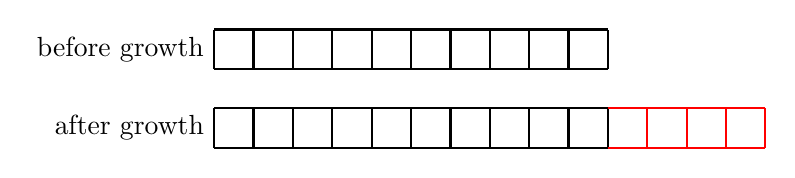
\begin{tikzpicture} [field/.style = {thick,step=5mm} ]
    \draw[field] (0mm,0mm) node[anchor = east,yshift=+2.5mm] {before growth} grid (50mm,5mm); 
    \draw[field] (0mm,-10mm) node[anchor=east,yshift=+2.5mm] {after growth} grid +(50mm,5mm);
    \draw[field,color=red] (50mm,-10mm)  grid +(20mm,5mm);
    \end{tikzpicture}
\end{minipage}
\caption{{\small\label{fig:field:growth1d} Growing a one dimensional field 
by $4$ elements.}}
\end{figure}
%%%---------------------------------------------------------------------------

%%%---------------------------------------------------------------------------
\begin{figure}[tb]
    \begin{minipage}[c]{0.3\linewidth}
        \begin{cppcode}
h5::nxfield f = ...;
//..... code omitted .....
f.grow(1,4);
        \end{cppcode}
    \end{minipage}
    \hfill
    \begin{minipage}[c]{0.65\linewidth}
        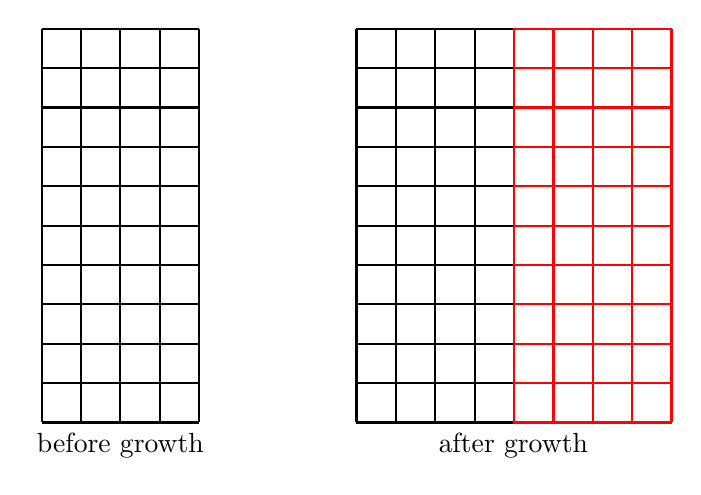
\begin{tikzpicture} [field/.style = {thick,step=5mm} ]
        \draw[field] (0mm,0mm) node[anchor = north,xshift=10mm] {before growth} grid (20mm,50mm); 
        \draw[field] (39.9mm,0mm) node[anchor=north,xshift=20mm] {after growth} grid +(20mm,50mm);
        \draw[field,color=red] (59.9mm,0mm)  grid +(20.1mm,50mm);
        \end{tikzpicture}
    \end{minipage}
    \caption{{\small\label{fig:field:growth2d} Growing a two dimensional field
    by $4$ elements along its second dimension.}}
\end{figure}
%%%---------------------------------------------------------------------------
The reason why there are no purely scalar fields is that during an experiment 
one would append data to a field as the measurement progresses. 
For this purpose \nxfield\ provides a \cpp{grow()} method which allows to 
extend the field along a particular dimension. The member function has the 
signature
\begin{cppcode}
void grow(size_t e,size_t n=1)
\end{cppcode}
where the first (mandatory) argument is the index of the dimension along which
the field should grow and the second (optional) argument contains the number of 
elements by which to grow. Figures~\ref{fig:field:growth1d} and
\ref{fig:field:growth2d} show examples of growing a one and a two dimensional
field respectively.

The canonical application for this feature would be to add content to a field 
as an experiment progresses. Using such a pattern we can start with a field 
of $0$ size and then add points if required. The principal code would look like
this
\begin{cppcode}
h5::nxfile f = ...;
h5::nxfield data = detector_group.create_field<uint16>("spectra",
                                                       shape_t{0,1024});
size_t index = 0;
while(true)
{
    data.grow(0,1); //grow by one element along first dimension
    //...... code omitted ....
}
\end{cppcode}
Note here that the initial shape of the field is $(0,1024)$. Such a pattern 
removes the burden of determining the number of points, recorded during 
an experiment, before the experiment starts. If the measurement is stopped 
somewhere in between the number of points written to the file matches exactly
the number of points recorded.  
It is important to note that one cannot extend the size of a field only along
\emph{existing} dimensions. It is not possible to change the rank of a field via
the growth method. Every attempt to do so will raise an \cpp{index\_error}
exception.
How to write the data will be explained in the next section.

%%%===========================================================================
\subsection{Partial reading and writing}

The previous section explained how to adjust the size of fields dynamically. 
What is still missing is how to write data to such a growing field. The 
\cpp{read()} and \cpp{write()} member functions used so far are always writing
the entire content of the field. This is not really what we want. 
Thus, \libpniio s \nxfield\ type provides partial IO quite similar to the 
\cpp{mdarray} template of \libpnicore. 

The best way to understand partial IO is to have a look on an example. We thus
will complete the previous one 

\begin{cppcode}
h5::nxfile f = ...;
h5::nxfield data = detector_group.create_field<uint16>("spectra",
                                                       shape_t{0,1024});
auto buffer = dynamic_array<uint16>::create_array(shape_t{1024});

size_t index = 0;
while(true)
{
    data.grow(0,1); //grow by one element along first dimension
    //...... code omitted ....

    //write data
    data(index++,slice(0,1024)).write(buffer);
}
\end{cppcode}
The important line of code here is the last one in the \cpp{for}-loop. To obtain
a selection of a field we can use the \cpp{()} operator of \nxfield. 
The selection works the same as for \cpp{mdarray}. However, the return value is 
a new field instance with the selection set. One currently cannot apply more
selections successively. 


%%%===========================================================================
\subsection{Field inquiry}\label{section:field:inquiry}

Fields share a set of inquiry functions with groups. These are \cpp{name()}, 
\cpp{filename()}, and \cpp{is\_valid()}. In addition to these functions
there are also some member functions which are special for fields. 
The \cpp{size()} member function returns the total number of elements 
stored in a field. If a selection has been applied to the field \cpp{size()}
returns the total number of elements selected. 
\cpp{type\_id()} returns the Id of the field elements data type. 
The \cpp{shape()} template function returns a container, which can be passed as
a template parameter, with the number of elements along each dimension. 
\begin{cppcode}
h5::nxfield field = ...;
auto s = field.shape<shape_t>();
\end{cppcode}



%%%===========================================================================
\section{Working with attributes}

Attributes are quite similar to fields. They can be attached to either a group
or a field to provide additional information (metadata) for a particular field
or group. Unlike fields attributes cannot 
\begin{itemize}
\item use compression
\item grow.
\end{itemize}
HDF5 attributes also do not support partial IO. However, \libpniio\ provides
partial IO for attributes in its implementation.
Attributes can be accessed from their parent object (field or group instance)
via the public attribute \cpp{attributes}. \cpp{attributes} is an instance of 
the \cpp{nxattribute\_manager} template class. The details about
\cpp{nxattribute\_manager} is only of interest for developers working on
\libpniio\ and hence will not be discussed here. Only the interface
\cpp{nxattribute\_manager} exposes is of interest and will be discussed in this
section. 

%%%===========================================================================
\subsection{Creating attributes}

Attributes are created via the \cpp{create()} template member functions 
provided by \cpp{nxattribute\_manager}. These functions are quite similar to
those used to create fields below groups. 
\begin{cppcode}
h5::nxfield f = ....;
auto units = f.attributes.create<string>("units");
\end{cppcode}
This short snippet creates an instance of \cpp{nxattribute} the template 
type used to represent attributes in memory. The newly created attribute 
is scalar and can store a single string. 
Multidimensional attributes can be constructed by adding a container with 
shape information to the argument list of the \cpp{create} template.
\begin{cppcode}
h5::nxfield f = ...;
auto matrix = f.attributes.create<float32>("transformation",shape_t{3,3});

std::cout<<matrix.rank()<<std::endl; //output is 2
\end{cppcode}
It is important here to note that even a scalar attribute has a rank of $1$. 
This might not be the obvious choice but makes fields and attributes more 
consistent. To check if an attribute is a scalar one could use the \cpp{size()}
member function of an attribute. If the \cpp{size()} returns $1$ the attribute
can be considered as scalar.

When one tries to create an attribute on an object which already has an
attribute of the same name an \cpp{object\_error} exception will be thrown. 
\begin{cppcode}
h5::nxfield f = ....;
f.attributes.create<string>("units"); //create the original attribute
f.attributes.create<float32>("units"); //would throw object_error
\end{cppcode}
However, an attribute can be overwritten with 
\begin{cppcode}
h5::nxfield f = ....;

//create the original attribute
f.attributes.create<string>("units"); 

//overwrite original attribute
f.attributes.create<float32>("units",true); 
\end{cppcode}
where the last argument of the second call to \cpp{create()} allows to 
overwrite an existing attribute. A similar call exists for multidimensional 
attributes
\begin{cppcode}
h5::nxfield f = ....;

//create the original attribute
f.attributes.create<string>("units",shape_t{3});       

//replace the original "units" attribute
f.attributes.create<float32>("units",shape_t{3,4},true); 
\end{cppcode}

%%%===========================================================================
\subsection{Attribute inquiry}

Attributes and fields share the same set of inquiry methods. Thus, see 
Section~\ref{section:field:inquiry} for details.

%%%===========================================================================
\subsection{Accessing an objects attributes}

The attribute manager instance associated with each field or group exposes a
very minimalistic but STL compliant container interface. 
Its \cpp{size()} returns the number of attributes attached to an object. 
One can access each attribute either by its index
\begin{cppcode}
h5::nxgroup g = ....;

for(size_t i=0;i<g.attributes.size();++i) 
    std::cout<<g.attributes[i].name()<<std::endl;
\end{cppcode}
or by its name
\begin{cppcode}
h5::nxgroup g = ....;
auto attr = g.attributes["NX_class"];
\end{cppcode}
When using the \cpp{[]} operator with a numeric index an \cpp{index\_error}
exception will be thrown if the index exceeds the total number of attributes. 
Similarly, \cpp{[]}, when used with an attributes name, will throw a
\cpp{key\_error} exception.
One can also iterate over all attributes, either by using the standard 
\cpp{begin()} and \cpp{end()} functions to retrieve iterators, or by using the
more modern for-each construction
\begin{cppcode}
h5::nxfield f = ....;
for(auto attr: f.attributes)
    std::cout<<attr.name()<<std::endl;
\end{cppcode}


%%%===========================================================================
\subsection{Reading and writing data from and to attributes}

Data IO for attributes works exactly the same as for fields with the exception
that attributes cannot be changed in size. 
A simple example for writing and reading a string attribute would look like this
\begin{cppcode}
string unit = "nm";
h5::nxfield f = ....;
auto attr = f.attributes.create<string>("units");
attr.write(unit);
//...... code omitted ......
attr.read(unit);
\end{cppcode}
The read/write member functions also accept instances of the \cpp{mdarray}
template as well as of \cpp{array}. Like for fields a pointer version exists 
to interact safely with legacy C libraries
\begin{cppcode}
size_t size = 9;
double *matrix = get_matrix_from_c_code();

h5::nxfield f = ....;
auto attr = f.attributes.create<float64>("matrix",shape_t{3,3});
attr.write(n,matrix);
\end{cppcode}
Reading works pretty much the same, however, you have to allocate memory before
reading the data from the attribute
\begin{cppcode}
h5::nxfield f = ....;
auto attr = f.attributes["matrix"]; //obtain the attribute from the field
float64 *matrix = allocate_memory(attr.size());

attr.write(attr.size(),matrix);
\end{cppcode}
Unlike standard HDF5 attributes support \libpniio's \nexus-attributes partial
IO. Partial IO with attributes works exactly the same way as with field
\begin{cppcode}
h5::nxfield f = ...;
auto attr = f.attributes.create<float64>("matrix",shape_t{3,3});
auto row  = dynamic_array<T>::create(shape_t{3});
//........... code omitted .......
for(size_t i=0;i<3;++i)
{
    row = .....; //fill row buffer with data
    attr(i,slice(0,3)).write(row);
}
\end{cppcode}
For reading data just replace the \cpp{write} with \cpp{read}. It should be
mentioned that using partial IO on attributes, though it works, can be
significantly slower than writing the entire attribute in a single step. 

%%%===========================================================================

\subsection{Attribute management}

There are two functions left of the \cpp{nxattribute\_manager} interface. 
One is the \cpp{exists()} member function which can be used to check for the
existence of a particular attribute. 
\begin{cppcode}
if(!field.attributes.exists("units"))
    std::cerr<<"Field does not have a units attribute!"<<std::endl;
\end{cppcode}
An attribute can be removed from an object using the \cpp{remove()} method. 
\begin{cppcode}
if(field.attributes.exists("units"))
    field.attributes.remove("units");
\end{cppcode}
The \cpp{remove} method throws \cpp{key\_error} if the attribute to delete does
not exists.





\FloatBarrier

%%%---------------------------------------------------------------------------
\chapter{Using algorithms}
\FloatBarrier

%%%---------------------------------------------------------------------------
\chapter{\nexus\ and XML}
%%%documentation concerning the XML functions

As \nexus\ organizes data objects in a tree like manner, XML is the obvious ASCII
representation for a \nexus\ file.
\libpniio\ thus provides a small but powerful set of functions to read and write 
\nexus\ data objects from and to XML files. The framework is based on the 
\cpp{boost::property\_tree} library. Clearly, the XML functionality provided 
by \libpniio\ does in no case replace a full XML parser. For instance, there are
no functions provided to manipulate the the XML content returned from 
any of the functions. However, as the \cpp{node} type used to represent 
XML data is an alias for the \cpp{boost::property\_tree} node type, one can use
functions from \cpp{boost::property\_tree} to do some additional work with the
XML results.
\libpniio\ provides two interfaces\
\begin{itemize}
\item a high level interface which consists of basically two functions. The high
level interface is described in section~\ref{sec:xml:highlevel}
\item And a low level interface -- these are the classes and functions used to
build the high level interface (described in section~\ref{sec:xml:lowlevel}).
\end{itemize}
Aside from this there are some simple functions which are common to both
interfaces and described in section~\ref{sec:xml:basic}.

%%%---------------------------------------------------------------------------
\section{Use cases}\label{sec:xml:usecases}

XML is a powerful and mature technology for representing structured data in 
ASCII. Though it has received some competitors like JSON, when it comes to 
complex structures XML is still the tool of choice\footnote{In fact, JSON
becomes quickly virtually unreadable if the structure becomes too deeply
nested.}
In this section some use cases for \nexus\ and XML will be presented. 

\subsection{Standard compliance verification of a file}

An always recurring request is the possibility to check a \nexus\ file with
respect to its compliance to the current standard. As the \nexus\ standard 
itself is defined in XML it would be reasonable to create an XML representation
of the file to check and use one of the available XML validation tools to 
verify the compliance of the file towards a particular standard. 
Using the XML representation of the file instead of the file directly has 
several advantages 
\begin{itemize}
\item being rather small, the XML representation can also be transfered 
over the network using a remote service for validation
\item it is at least in principle human readable 
\item many of the required tools already exist. 
\end{itemize}
On step in this entire process is to convert a \nexus\ file to its ASCII XML 
representation.

\subsection{Generating \nexus\ structures from XML}

The structure of a \nexus\ file can become rather complex. In a rather complex 
environment like at a synchrotron beamline it would be naive to use static 
code to create the file. A more feasible approach would be to implement 
generic code which generates the structure of a file from an XML template. 
The template could be generated either manually by the user or by means 
of another program written in whatever language is reasonable for this purpose. 

\subsection{Metadata ingestion of a file}

In some situations a $3$rd party may needs to process some of the metadata 
stored in the file while not having access to the file. One possible application
would be a data catalogue. Instead of making the file available the XML dump 
of the \nexus\ file could be sent to the system while moving the \nexus\ file 
to its final location on the storage system.

%%%---------------------------------------------------------------------------
\section{Basic XML handling}{\label{sec:xml:basic}

All XML related functions and classes resided within a separate namespace 
\cpp{pni::io::nx::xml}. An XML document is represented by an instance of 
type \cpp{node}. \cpp{node} is an alias for \cpp{boost::property\_tree::ptree}. 
Thus it can be used along with all functions an methods provided by the 
\cpp{ptree} type provided by \cpp{boost::property\_tree}. Aside from the 
functionality from \cpp{boost::property\_tree} \libpniio\ provides some 
\nexus\ related convenience functions. 

An instance of \cpp{node} can be created either from a string
\begin{cppcode}
    xml::node n = xml::create_from_string(xmldata);
\end{cppcode}
where \cpp{xmldata} is a string with the XML content, 
or from a file
\begin{cppcode}
    xml::node n = xml::create_from_file(fname);
\end{cppcode}
where \cpp{fname} is a string with the name of the file. Both functions 
return the root node of the XML document. See the \cpp{property\_tree}
documentation in the \cpp{BOOST} distribution for more information what one can
do with such an object. For the rest of this chapter no additional knowledge
about \cpp{BOOST}s \cpp{property\_tree} library is required.
To write the content of a node to a stream one can use the default 
output stream operator
\begin{cppcode}
    xml::node n = ....;
    std::cout<<n<<std::endl;
\end{cppcode}


%%%===========================================================================
\section{High level XML interface}\label{sec:xml:highlevel}

The high-level XML interface basically consists of two function templates 
\begin{description}
\item[xml\_to\_nexus] which creates \nexus\ objects from XML templates
\item[nexus\_to\_xml] which generates XML from \nexus\ objects.
\end{description}
Additionally there are some convenience functions available. All of this will be
described in more detail in this section.

%%%---------------------------------------------------------------------------
\section{\nexus\ objects from XML}\label{sec:xml::nxtoxml}

Creating \nexus\ objects from XML might be the most common operation performed 
by this part of the library. The next example illustrates the most common 
use case 
\begin{cppcode}
#include <pni/io/nx/nx.hpp>
#include <pni/io/nx/xml.hpp>

using namespace pni::io::nx;

int main(int argc,char **argv)
{
    xml::node n = ....;
    h5::nxfile f = ....;
    h5::nxgroup root = f.root();
    
    xml::xml_to_nexus(n,root);

    return 0;
}
\end{cppcode}
Here, the structure of a \nexus\ tree is described by XML and then converted 
to \nexus\ by means of the \cpp{xml\_to\_nexus} function. The first argument 
of this function is the XML node while the second is the parent object 
below which the new structure should be created. All data already available 
in the XML file will be stored in the fields and attributes of the created
\nexus\-tree. 


%%%---------------------------------------------------------------------------
\subsection{XML from \nexus\ objects}\label{sec:xml:xmltonx}

The work horse for \nexus\ to XML conversion is the \cpp{nexus\_to\_xml} function
template. The most probably simplest use case is demonstrated in the next
example 
\begin{cppcode}
#include <pni/io/nx/nx.hpp>
#include <pni/io/nx/xml.hpp>

using namespace pni::io::nx;

int main(int argc,char **argv)
{
    h5::nxfile f = ....;
    h5::nxgroup root = f.root();

    xml::node root_node;
    xml::nexus_to_xml(root,root_node);
    std::cout<<root_node<<std::endl;

    return 0;
}
\end{cppcode}
Here, the entire structure of the \nexus\ file is stored below the XML root node 
which is at the end dumped to standard output.
This simple example already raises an important question: how to deal with the
data stored in the \nexus\ file. As \nexus\ files can be used to store large amounts
of data it would not be wise to convert all this data to ASCII (think about a 3D
image stack stored in the file). However, some data might be required. 
The \cpp{nexus\_to\_xml} template thus provides a third optional argument which 
is a predicate function which decides for which field or attribute data will be
written to the file. 
The signature of the predicate is 
\begin{minted}[fontsize=\small]{cpp}
template<
         typename GTYPE,
         typename FTYPE,
         typename ATYPE
        >
bool predicate(const nxobject<GTYPE,FTYPE,ATYPE> &o);
\end{minted}
The function returns \cpp{true} if the data of a particular object should be 
included in the XML output. 
It is wise to not make this function to specific. Thus, the name of a field 
is not a good criterion for deciding whether or not to write data. 
A much better approach is to check for certain properties of an object. 
For the previous example a possible predicate could look like this
\begin{cppcode}
//code omitted 
bool write_scalars(const h5::nxobject &o)
{
    if(is_field(o) || is_attribute(o))
    {
       return size(o)==1;
    }
    else 
        return false;
}

int main(int argc,char **argv)
{
    //code omitted 
    xml::nexus_to_xml(root,root_node,write_scalars);

    //code omitted
    return 0;
}
\end{cppcode}
This predicate determines that only the data from fields and attributes 
is written to the XML tree if their size is equal to $1$ (in other words -- only
scalars are written to the file). 
Such an approach keeps the resulting XML document small while using a rather 
general predicate which would match quite a lot of use cases. The default 
policy is to write no data.


%%%===========================================================================
\section{The XML low level interface}\label{sec:xml:lowlevel}



\FloatBarrier

%%%---------------------------------------------------------------------------
\appendix
\chapter{Parsing ASCII data}\label{appendix:parsers}

In times of binary data formats like Nexus it seems anachronistic to devote an
entire chapter of the appendix to the problem of ASCII parsing. However, 
ther are several good reasons why one should care about correctly reading 
ASCII data (in particular numbers)
\begin{enumerate}
\item for historical reasons there is a lot of legacy ASCII data out there which
may should be processed -- for this reason alone it is necessary to deal with
ASCII data in a reasonable way.
\item uses still provided input to programs via ASCII files (for instance using
XML) or via the command line -- in both cases the program has to process these
files correctly. 
\item even input fields in GUI toolkits typically return the data entered by 
the user as an characater string which must be parsed in order to obtain a 
numerical value.
\end{enumerate}

One crucial aspect when processing ASCII data is number parsing.
This chapter will describe in more detail the parser framework provided by 
\libpniio. 

All parsers basically utilize two exceptions to denote errors
\begin{description}
\item[\texttt{parser\_error}] which is thrown in situations where the ASCII 
representation is malformed, or
\item[\texttt{range\_error}] which is thrown when the ASCII string is well 
formatted but the numeric range represented by the number exceeds the 
target type {\bf not yet implemented}
\end{description}
This information should be sufficient to recognize the error in the input data. 
Before discussing the individual functions and types provided by \libpniio\ 
for parsing ASCII a thorough discussion of the ASCII representations of 
the primitive data types will be made.

%%----------------------------------------------------------------------------
\section{ASCII representations of primitive data types}

\subsection{Integers and floating point numbers}
The ASCII representations of integer and floating point numbers follow the 
C++ standard conventions and will not be discussed here in greater detail.

\subsection{Complex numbers}

Complex numbers can be represented in two forms: as real and imaginary part 
or as imaginary part only. A real-part only representation is not possible 
as such a number would be indistinguishable from a simple floating point type. 
The full representation (real and imaginary part) looks somehow like this
\begin{align}
A \pm K B
\end{align}
where $A$ and $B$ are denoting the real and imaginary part respectively. 
$K$ is the symbol which denotes the complex unit $\sqrt{-1}$. This can be either
$i$, $j$, or $I$. To given an example 
\begin{verbatim}
1.2+j3.4
\end{verbatim}
would be a valid complex number while
\begin{verbatim}
1.2+J2.4
\end{verbatim}
not. It is important to not that the sign between the real- and imaginary-part 
must not be surrounded by blanks. Furthermore, the imaginary part must not have
an extra leading sign as its sign is already determined by the sign between
real- and imaginary part. 
A imaginary-part only number would look like this
\begin{verbatim}
+i3
\end{verbatim}
where the sign in front of the complex unit is optional and could have been 
omitted in this particular case 
\begin{verbatim}
i3
\end{verbatim}

\subsection{Boolean values}

The two boolean values \cpp{true} and \cpp{false} are represented exactly in
this way as ASCII strings. Be aware that the syntax is case sensitive. Thus 
\cpp{True} or \cpp{False} would cause a \cpp{parser\_error}.

%%----------------------------------------------------------------------------
\section{Parser rules}




\FloatBarrier

%%%---------------------------------------------------------------------------
\chapter{\nexus-XML serialization}

\libpniio\ uses XML an XML dialect very similar to NXDL in order to serialize
\nexus-objects. The deviations from NXDL are due to the fact that \libpniio\ has
to build or dump concrete objects to XML rather than describing the fundamental
properties (as NXDL does). 
A good example here is the data type. NXDL uses \cpp{NX\_FLOAT} to denote that a
field or attribute has to be a floating point type. However, it does not
prescribe which one to use. For the purpose of NXDL this is not of importance -
the data type must be any of the available floating point types. 
\libpniio, on the oder side, needs to write objects to as well as to construct
objects from XML. Hence, a type like \cpp{NX\_FLOAT} would be too general. 

%%%===========================================================================
\section{Common deviations from NXDL}

This section deals with those deviations from NXDL which are common too all
objects in the \nexus-universe. 

\subsection{Data types} 

While NXDL uses general type descriptors like \cpp{NX\_FLOAT} or \cpp{NX\_CHAR} 
, which are more closely related to \libpnicore s type class concept, \libpniio\ 
uses the string representation of data types as described by the \libpnicore\
users guide. For a field one may uses 
\begin{minted}[fontsize=\small]{xml}
<field name="data" type="float32"/>
\end{minted}
where \cpp{float32} tells \libpniio\ exactly which floating point type to use.
Strings are represented by \cpp{string} instead of \cpp{NX\_CHAR}.

\subsection{Enumerations}

\libpniio\ does not support enumerations. An enumeration in NXDL lists the 
possible values a particular field or attribute can take. However, for
\libpniio\ the objects already has a particular state when it is written to XML
or has to be constructed in a particular state when read from XML. 
Enumerations thus would not make too much sense.

\subsection{Data in XML content} 

Unlike NXDL, \libpniio allows data to be stored in the XML output. This is 
particularly useful for scalar and rather small arrays of numeric data 
and strings. For numeric data all features are allowed. Data from multi
dimensional fields can easily be stored and read to and from XML. 
The data is simple dumped as a linear sequence of string representations of the 
numeric values separated by whitespace characters. 
As the dimensions of a multi dimensional field is stored in a special tag 
the field can easily constructed from the linear storage.

\subsubsection{The special case of strings} 

Strings are difficult. Thus only scalar string data can be currently stored. 
The reason for this is simple. While the ASCII representations of numeric data
can easily separated by whitespace characters, this is no longer the case for
strings. The whitespace maybe part of a single element. In other words, it is 
unclear what the delimiter characters are. 

\subsubsection{Binary data}

%%%===========================================================================
\section{XML attribute representation}

Attributes have to be represented by a dedicated tag if they are not mandatory
for a particular tag type. For instance the \cpp{group} and \cpp{type} attribute
are mandatory for virtually all objects and are thus always part of a tag. 
However, the \cpp{transformation\_type} attribute is optional for a \cpp{field}
tag and thus has to be encoded in a separate attribute tag. 

%%%---------------------------------------------------------------------------
\subsection{Scalar attributes}
\begin{xmlcode}
<attribute name="transformation_type" type="string"> rotation </attribute>
\end{xmlcode}
The \cpp{name} and \cpp{type} attributes have their obvious meaning and do not
need extra explanation. 
The data is kept in the \cpp{CDATA} section of the tag and needs to be parsed 
in case of reading.

%%%---------------------------------------------------------------------------
\subsection{Multidimensional attributes}

As of the NIAC meeting at the APS in December 2014 Nexus officially supports

\begin{xmlcode}
<attribute name="vector" type="float32">
    <dimensions rank="1">
        <dim value="3" index="1"/>
    </dimensions>
    0 1 0 
</attribute>
\end{xmlcode}

More interesting, how to manage multidimensional strings 
\begin{xmlcode}
<attribute name="log" type="string">
    <dimensions rank="1">
        <dim value="4" index="1"/>
    </dimensions>
    "line 1: blablabla" "line2: blablabla" 
    "line 3: more text" "line 4: the last line"
</attribute>
\end{xmlcode}
Strings must be stored quoted. This is important for the case of
multidimensional arrays as it would be hard otherwise to define a delimiter 
between the different strings. As a consequence it is not possible to store 
strings which contain a \".

%%%===========================================================================
\section{XML field representation}

%%%---------------------------------------------------------------------------
\subsection{Scalar fields}

\begin{xmlcode}
<field name="integral" type="uint16" units="cps"> 102 </field>
\end{xmlcode}
The attributes \cpp{name} and \cpp{type} have the same meaning as for 
attributes. More interesting is the \cpp{units} attribute as its meaning 
differs from NXDL. In NXDL the \cpp{units} attribute describes the 
dimension (length, angular, etc.) while in our serialization approach 
it represents a physical units. In this case this would be \emph{counts by 
second} (\cpp{cps}).

%%%---------------------------------------------------------------------------
\subsection{Multidimensional fields}

Multidimensional fields are described like multidimensional attributes 
\begin{xmlcode}
<field name="rotmat" type="float64" units="a.u.">
    <dimensions rank="2">
        <dim index="1" value="3"/>
        <dim index="2" value="3"/>
    </dimensions>
    1 2 3
    4 5 6
    7 8 9
</field>
\end{xmlcode}
Unfortunately this is not enough when we consider HDF5 as a storage backend. 
We definitely need more information.

%%%---------------------------------------------------------------------------
\subsection{Adding chunking}

The first thing required for HDF5 is that we have to store chunk information. 
\begin{xmlcode}
<field name="images" type="uint16" units="a.u.">
    <dimensions rank="3">
        <dim index="1" value="0"/>
        <dim index="2" value="1024"/>
        <dim index="3" value="2048"/>
    </dimensions>
    <chunk rank="3">
        <dim index="1" value="1"/>
        <dim index="2" value="1024"/>
        <dim index="3" value="2048"/>
    </chunk>
</field>
\end{xmlcode}

%%%---------------------------------------------------------------------------
\subsection{Adding compression}

\begin{xmlcode}
<field name="images" type="uint16" units="a.u.">
    <dimensions rank="3">
        <dim index="1" value="0"/>
        <dim index="2" value="1024"/>
        <dim index="3" value="2048"/>
    </dimensions>
    <chunk rank="3">
        <dim index="1" value="1"/>
        <dim index="2" value="1024"/>
        <dim index="3" value="2048"/>
    </chunk>
    <filters>
        <filter index="1" name="fletcher32"/>
        <filter index="2" name="deflate">
            <param name="rate"> 8 </param>
        </filter>
    </filters>
</field>
\end{xmlcode}




%\bibliography{libpniio_ug}

\end{document}
